\section{Trực quan hóa dữ liệu với Kibana}
Trong phần này, chúng ta sẽ điểm qua những tính năng chính (trực quan hóa) của Kibana bằng cách khám phá tập dữ liệu mẫu (sẵn có của Elasticsearch) và xây dựng dashboard trên các tập dữ liệu này.

\begin{figure}[H] % places figure environment here   
    \centering % Centers Graphic
    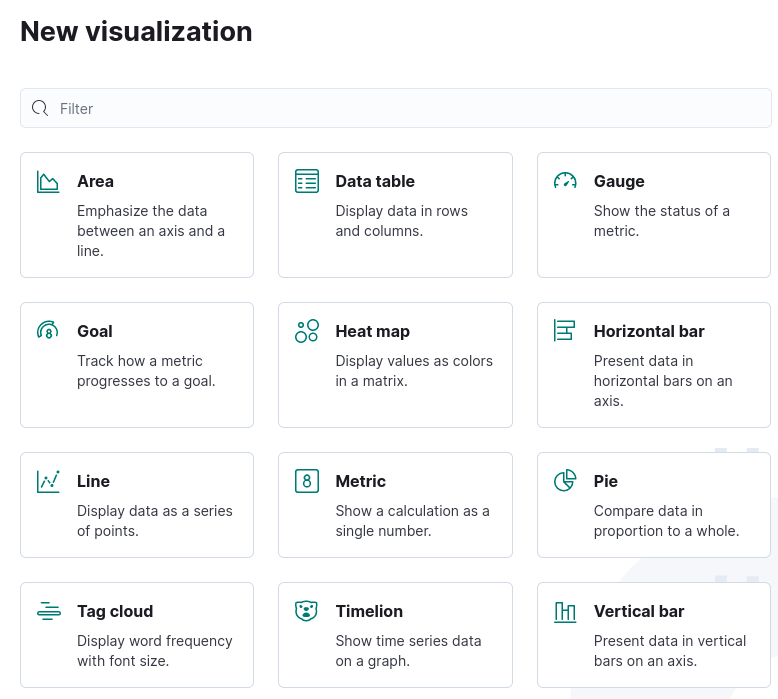
\includegraphics[width=1\textwidth]{figures/kibana_charts.png} 
    \caption{Các biểu đồ được Kibana dựng sẵn} % Creates caption underneath graph
    \label{fig:elk_01}
\end{figure}

Với một ứng dụng cổ điển, thường thì các lập trình viên sẽ phải xây dựng một trang web quản trị riêng nhằm cung cấp các biểu đồ trực quan để admin nắm được những thông tin cần thiết. Tuy nhiên việc này là khá tốn kém chi phí và công sức do người lập trình ngoài việc phải code phần giao diện còn phải xây dựng các API cần thiết cũng như ghi vào cơ sở dữ liệu các thông tin theo yêu cầu để hiển thị. Kibana giảm thiểu công sức cho chúng ta rất nhiều bằng cách cung cấp sẵn những biểu đồ đủ các thể loại từ biểu đồ diện tích, biểu đồ nhiệt, biểu đồ cột, biểu đồ đường, thậm chí cả biểu đồ địa lý... Mà quan trọng là ta không cần phải viết code hay truy vấn vào cơ sở dữ liệu (có thể dẫn đến quá tải hệ thống).

\begin{figure}[H] % places figure environment here   
    \centering % Centers Graphic
    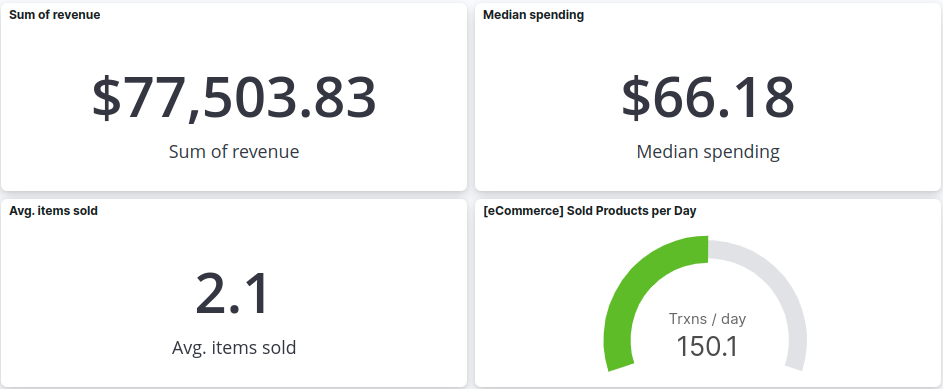
\includegraphics[width=1\textwidth]{figures/sum_reve.png} 
    \caption{Bảng tổng hợp lợi nhuận (\textit{tập dữ liệu eCommerce dựng sẵn của Elasticsearch})} % Creates caption underneath graph
    \label{fig:elk_01}
\end{figure}

Để nắm tổng quan về tình hình kinh doanh, người quản trị có thể theo dõi biểu đồ tổng hợp với những con số được làm nổi bật.

\begin{figure}[H] % places figure environment here   
    \centering % Centers Graphic
    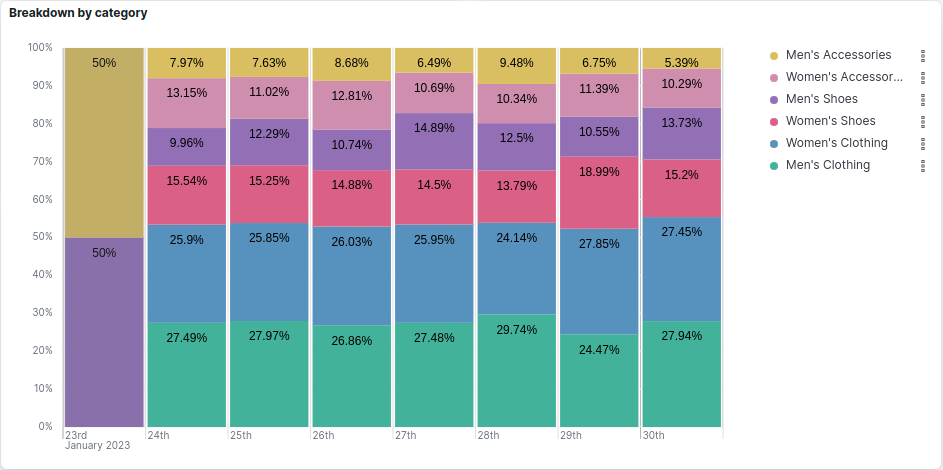
\includegraphics[width=1\textwidth]{figures/ecom_cat.png} 
    \caption{Một biểu đồ đơn giản thể hiện phần trăm các loại mặt hàng được bán theo ngày của một website bán hàng trực tuyến (\textit{tập dữ liệu eCommerce dựng sẵn của Elasticsearch})} % Creates caption underneath graph
    \label{fig:elk_01}
\end{figure}

Nhìn vào biểu đồ, người quản trị có thể nắm được thông tin tổng quan là mặt hàng quần áo nam và nữ được bán với tỉ trọng lớn và khá đều đặn qua các ngày. Trong khi đó mặt hàng phụ kiện thì bán được khá ít. Lớp phủ màu được sử dụng để người xem dễ theo dõi tỉ trọng của mặt hàng. Ngoài ra tại mỗi khối, tỉ trọng cũng được ghi dưới dạng phần trăm để người xem nắm được con số cụ thể. 

\begin{figure}[H] % places figure environment here   
    \centering % Centers Graphic
    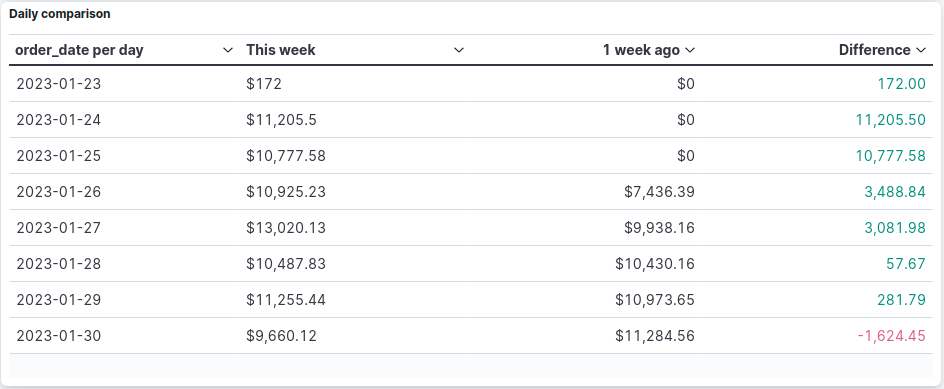
\includegraphics[width=1\textwidth]{figures/daily_compare.png} 
    \caption{So sánh doanh thu của tuần này và tuần trước (\textit{tập dữ liệu eCommerce dựng sẵn của Elasticsearch})} % Creates caption underneath graph
    \label{fig:elk_01}
\end{figure}

Một ví dụ khác về việc áp dụng màu sắc và con số. Màu xanh thể hiện doanh thu tăng và ngược lại màu đỏ thể hiện sự sụt giảm doanh thu. Từ đó người quản trị có thể điều tra nguyên nhân và đưa ra quyết định kinh doanh phù hợp.

Kibana là một tool khá mạnh về biểu diễn dữ liệu hướng thời gian bởi lý do rất tự nhiên, trong thực tế doanh nghiệp thường sử dụng ELK làm hệ thống quản lý log mà log là một loại dữ liệu hướng thời gian điển hình. Một trong số những độ đo quan trọng nhất mà một website hay một ứng dụng web cần quan tâm đó là phản hồi của ứng dụng với yêu cầu từ khách hàng (\textit{http status}). 

\begin{figure}[H] % places figure environment here   
    \centering % Centers Graphic
    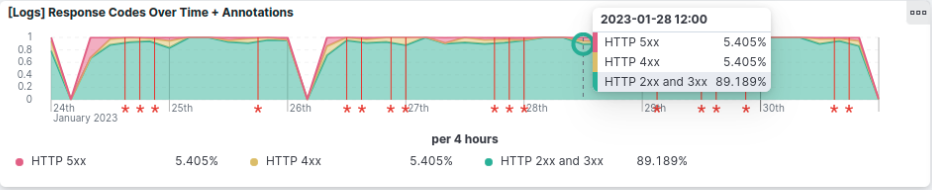
\includegraphics[width=1\textwidth]{figures/req_http_stt.png} 
    \caption{ HTTP Status của một ứng dụng web (\textit{tập dữ liệu Web Traffic dựng sẵn của Elasticsearch})} % Creates caption underneath graph
    \label{fig:elk_01}
\end{figure}

Chúng ta thường kì vọng số lỗi 4xx hoặc 5xx là ít nhất có thể, đặc biệt là 5xx (các lỗi hệ thống). Bởi lẽ lỗi 500 là đại diện của sự mất kiểm soát, có thể trong quá trình lập trình ta không bắt hết các ngoại lệ hay ứng dụng bị crash, dịch vụ ngoài chết... Đây được coi là lỗi nguy hiểm mà ta cần ứng cứu ngay lập tức. Kibana cung cấp một biểu đồ theo thời gian rất trực quan mà chúng ta có thể quan sát thấy ngay những lỗi nguy hiểm (màu đỏ - do người xây dựng biểu đồ cấu hình). Ngoài ra ta cũng có thể tương tác với biểu đồ bằng cách giữ chuột ở một vị trí nhất định để biết được tỉ lệ của các mã phản hồi HTTP trong một khoảng thời gian nào đó. 

\begin{figure}[H] % places figure environment here   
    \centering % Centers Graphic
    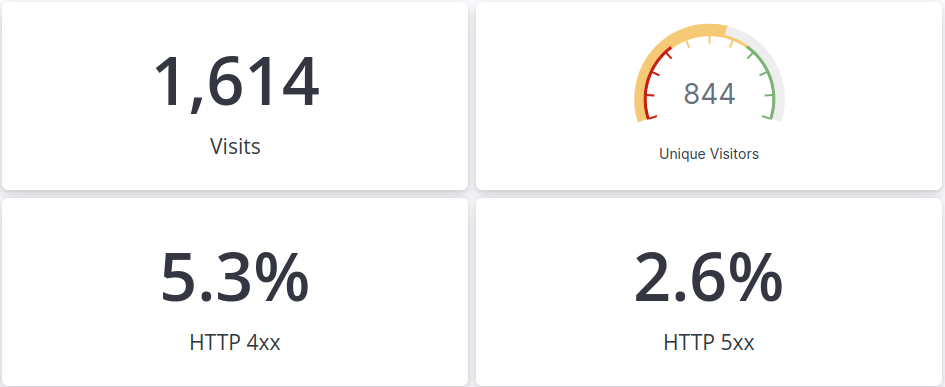
\includegraphics[width=1\textwidth]{figures/http_stt_sum.png} 
    \caption{ Tổng quan HTTP Status (\textit{tập dữ liệu Web Traffic dựng sẵn của Elasticsearch})} % Creates caption underneath graph
    \label{fig:elk_01}
\end{figure}

Tương tự ta cũng có thể xây dựng biểu đồ tổng quan để người dùng nắm được số HTTP Status đại diện cho lỗi trong khoảng thời gian cấu hình để có hướng điều tra hoặc cải thiện.